\documentclass[a4paper, 12pt]{fga}

% |--- T�tulos, autor, banca ---|----------------------{{{
\title{} % t�tulo na forma principal
\tituloficha{T�tulo para a ficha,\\\,[Distrito Federal], 2018.} % t�tulo na forma a constar da ficha
                                                  % catalogr�fica (incluir mudan�as de
                                                  % linha usando \\ quando necess�rio)
\titulocapaA{Generative Adversarial Network Prior Information}
\titulocapaB{for Improved Compressed Sensing}
\titulocapaC{Magnetic Resonance Image Reconstruction}

\titulofichadois{T�tulo para a ficha (parte 2)}
\author{Gabriel Gomes Ziegler}
\nomeinvertido{Ziegler, Gabriel}
\orientador{~Cristiano Jacques Miosso, PhD}
\coorientador{~Davi Benevides Gusm�o, MSc}
\data{December 2020}
\ano{2020}
\areaum{Deep Learning} % Preencher com termos escolhidos para identificar a �rea
\areadois{Magnetic Resonance Image Reconstruction}
\areatres{\emph{Compressive Sensing}}
\areaquatro{Generative Adversarial Network}
\endereco{gabrielziegler3@gmail.com}
\cep{CEP xxxxx-xxx}

\membrobancainterno{Prof. Jos� da Silva, PhD}
\membrobancaexterno{Prof. Jo�o da Silva, PhD}
%---}}}

% |--- Bibliotecas utilizadas ---|----------------------{{{
\usepackage[margin=1in]{geometry}
\usepackage{setspace}
\usepackage{multirow}
\usepackage{booktabs}
\usepackage[latin1]{inputenc}
\usepackage{enumerate}
\usepackage{xfrac}
\usepackage{color, colortbl}
\usepackage{placeins}
\usepackage[graphicx]{realboxes}
\usepackage{float}
\usepackage{subfig}
\usepackage{amsmath, amssymb}
\usepackage{rotating}
\usepackage{indentfirst}
\usepackage{multicol, blindtext, graphicx}
\usepackage[margin=0.40in,font=small,labelfont=bf,labelsep=period]{caption}
\usepackage{hyperref}
\usepackage[autostyle]{csquotes}
\hypersetup{
    colorlinks,
    citecolor=blue,
    filecolor=blue,
    linkcolor=black,
    urlcolor=blue
}
%---}}}

% |- Formato de refer�ncias (use apenas uma das 2 linhas seguintes; comente a outra) -|-{{{
\newcommand{\formatobibliografia}{numero}
%\newcommand{\formatobibliografia}{autorano}

\ifthenelse{\equal{\formatobibliografia}{numero}}{
\bibliographystyle{unsrt}
}
{}

\ifthenelse{\equal{\formatobibliografia}{autorano}}{
\usepackage{apalike}
\bibliographystyle{apalike}
}
{}
%---}}}

% |--- Espa�amento, configura��o de t�tulo de se��es ---|----------------------{{{
\onehalfspacing

\makeatletter
\renewcommand{\section}{\@startsection
{section}
{1}
{0mm}
{-\baselineskip}
{0.5\baselineskip}
{\large\bf}}
\makeatother

\makeatletter
\renewcommand{\subsection}{\@startsection
{subsection}
{2}
{0mm}
{-\baselineskip}
{0.5\baselineskip}
{\bf\sffamily}}
\makeatother

\makeatletter
\renewcommand{\subsubsection}{\@startsection
{subsubsection}
{3}
{0mm}
{-\baselineskip}
{0.5\baselineskip}
{\bf\sffamily}}
\makeatother

\setlength{\parindent}{20pt}
\setlength{\parskip}{12pt}
\newcommand{\spaceinitialsname}{0.4mm}
\newcommand{\porcento}{\scalebox{0.5}{~}\scalebox{0.9}{\%}}
\newcommand{\scanner}{\emph{scanner}}
\newcommand{\scanners}{\emph{scanners}}
\newcommand{\cmcubico}{${\textrm{cm}^{\scalebox{0.7}{3} }}$}
\setcounter{secnumdepth}{3}
%\setcounter{tocdepth}{3}
%---}}}

% |--- Comandos especiais ---|----------------------{{{
\newcommand{\cmquad}{${\textrm{cm}^{\scalebox{0.7}{2}} }$}
\newcommand{\mmquad}{${\textrm{mm}^{\scalebox{0.7}{2}} }$}
\newcommand{\gcmquad}{${\textrm{g}}/{\textrm{cm}^{\scalebox{0.7}{2}} }$}
\newcommand{\subsecref}[1]{Section~\ref{#1}}
\newcommand{\figref}[1]{Figure~\ref{#1}}
\newcommand{\etal}{\emph{et~al.}}
\newcommand{\Jawsonly}{{\emph{Jaws-Only}} }
\newcommand{\jawsonly}{{\emph{jaws-only}} }
\newcommand{\software}{\emph{software}}
\newcommand{\Section}[1]{\section{\textbf{#1} }}
\newcommand{\Sectionlabel}[2]{\section{\textbf{#1}\label{#2} }}
\newcommand{\percentagesignscale}{0.9}
\newcommand{\subsubsubsection}[1]{\vspace{16pt}\noindent\textbf{#1}\\[12pt]}
\newcommand{\commenttext}[1]{}
%---}}}

% |--- Diret�rio(s) com figuras (se desejar, inclua subdiret�rios) ---|-------------{{{
\graphicspath{{figuras/}}
%---}}}

% |--- Lista de palavras que n�o podem ser separadas em s�labas ---|------------------{{{
\hyphenation{development results Commissioning possibility Philadelphia Devic Calculations Calculation}
%---}}}

% |--- Texto principal ---|----------------------{{{
\begin{document}

\maketitle

% |--- Ep�grafe, dedicat�ria ---|----------------------{{{
% Se desejar uma ep�grafe, remova o % do in�cio das pr�ximas linhas (at� ==============)
%\clearpage
%\hspace{1mm}
%
%\vfill
%
%\hspace{1mm}
%
%\begin{center}
%\emph{Ep�grafe} \\
%Autor da ep�grafe
%\end{center}
%
%\hspace{1mm}
%
%\vfill
%
%\hspace{1mm}
% ==============

% Se desejar uma dedicat�ria, remova o % do in�cio das pr�ximas linhas (at� ==============)
%\clearpage
%\hspace{1mm}
%
%\vfill
%
%\begin{flushright}
%\begin{itshape}
%Texto da dedicat�ria.
%\end{itshape}
%\end{flushright}
% ==============
%---}}}

% |--- Agradecimentos ---|----------------------{{{
% Se desejar incluir agradecimentos, remova o % do in�cio das pr�ximas linhas (at� ==============)
% \clearpage
%\noindent{\bfseries{\maiusc{\large Agradecimentos}} }
%
%\vspace{24pt} Agradecimentos
%
%\noindent
%\clearpage
% ==============
%---}}}

% |--- Resumo e Abstract ---|----------------------{{{
\newgeometry{bottom=0.8in, top=0.9in, left=0.9in, right=0.9in}

%\noindent{\bfseries{\maiusc{\large Resumo}} }
%
%\vspace{12pt}
%A vers�o final do documento incluir� um resumo de todo o trabalho, incluindo metodologia, resultados e conclus�o.
\acresetall % Manter essa linha!
\clearpage
\restoregeometry
%\chapter{Abstract}
%\noindent{\bfseries{\maiusc{\large Abstract}} }
%
%\vspace{24pt}
%The final version of this document will include an abstract. This will summarize the introduction (contextualization, objectives, justification), the methodology, the results, and the conclusion.
\acresetall % Manter essa linha!
\indice
%---}}}

% |--- Lista de S�mbolos, Nomenclaturas e Abrevia��es ---|----------------------{{{
\begin{center}
	{\bfseries{\maiusc{\large Nomenclature and Abbreviations}} }%
\end{center}

\acrodef{MRI}[MRI]{Magnetic Resonance Imaging}
\acrodef{MR}[MR]{Magnetic Resonance}
\acrodef{ANN}[ANN]{Artificial Neural Networks}
\acrodef{DL}[DL]{Deep Learning}
\acrodef{ML}[ML]{Machine Learning}
\acrodef{GAN}[GAN]{Generative Adversarial Network}
\acrodef{CNN}[CNN]{Convolutional Neural Network}
\acrodef{GPU}[GPU]{Graphics Processing Units}
\acrodef{CV}[CV]{Computer Vision}
\acrodef{NLP}[NLP]{Natural Language Processing}
\acrodef{AI}[AI]{Artificial Intelligence}
\acrodef{CS}[CS]{Compressed Sensing}
\acrodef{MLP}[MLP]{Multilayer Perceptron}
\acrodef{DFN}[DFN]{Deep Feedforward Networks}
\acrodef{SNR}[SNR]{Signal-to-Noise Ratio}
\acrodef{SSIM}[SSIM]{Structural SIMilarity}
\acrodef{PSNR}[PSNR]{Peak Signal-to-Noise Ratio}
\acrodef{DCGAN}[DCGAN]{Deep Convolutional GAN}
\acrodef{ReLU}[ReLU]{Rectified linear units}
\acrodef{SGD}[SGD]{Stochastic Gradient Descent}

\begin{acronym}
	\acro{MRI}{Magnetic Resonance Imaging}
	\acro{MR}{Magnetic Resonance}
	\acro{ANN}{Artificial Neural Networks}
	\acro{DL}{Deep Learning}
	\acro{ML}{Machine Learning}
	\acro{GAN}{Generative Adversarial Network}
	\acro{CNN}{Convolutional Neural Network}
	\acro{GPU}{Graphics Processing Units}
	\acro{CV}{Computer Vision}
	\acro{NLP}{Natural Language Processing}
	\acro{AI}{Artificial Intelligence}
    \acro{CS}{Compressed Sensing}
    \acro{MLP}{Multilayer Perceptron}
    \acro{DFN}{Deep Feedforward Networks}
    \acro{SNR}{Signal-to-Noise Ratio}
    \acro{SSIM}{Structural SIMilarity}
    \acro{PSNR}{Peak Signal-to-Noise Ratio}
    \acro{DCGAN}{Deep Convolutional GAN}
    \acro{ReLU}{Rectified linear units}
    \acro{SGD}{Stochastic Gradient Descent}
\end{acronym}

\clearpage
%---}}}

% |--- Introduction ---|----------------------{{{
\chapter{Introduction}

In this thesis, we propose a \ac{GAN} approach for prior information extraction to feed a \ac{CS} algorithm, aiming to reconstruct images with both reduced signal-to-noise error and less acquisition time compared to conventional \ac{CS}.
Achieving higher quality with reduced number of samples allows faster exam procedures, making \ac{MRI} cheaper, faster and more convenient for both patients and clinics.

\section{Context}

\ac{MRI} is a widely used imaging modality in medical practice because of its great tissue contrast capabilities, it has evolved into the richest and most versatile biomedical imaging technique today~\cite{bryan_introduction_2009}, making \ac{MRI} the best option for medical imaging whenever it is possible to use.

However, like everything in life, there is a trade-off to consider when using \ac{MRI}.
Typically, reconstructing an \ac{MRI} is an ill-posed linear inverse task (a problem that has either none or infinite solutions in the desired class).
Problems of this nature impose a trade-off between \textit{accuracy} and \textit{speed}~\cite{kabanikhin_definitions_2008}.
The information obtained from \ac{MR} is commonly represented by individual samples in the k-space, which translates to the Fourier transform of the image to be reconstructed~\cite{miosso_compressive_2009-1}.
This \ac{MR} sampling sparse nature makes \ac{CS} a liable technique to use when reconstructing \ac{MRI}, hence we here propose a novel \ac{CS} prior information approach for better results.

\ac{CS} has been for years the state-of-art technique in \ac{MRI} reconstruction and has been improved later by the use of prior information~\cite{miosso_compressive_2009-1}.
\ac{CS} uses the premise that given a signal with a sparse representation in some known domain, it is possible to reconstruct the signal using limited linear measurements taken from a non-sparse representation.

\ac{ML} methods have been utterly developed and improved recently with the use of higher computing power derived from the invention of \ac{GPU} and other hardware improvements, allowing \ac{ANN} to come to practicality.
These \ac{ANN} models, often referenced as \ac{DL}, have become the state-of-art in various areas, such as \ac{CV}, \ac{NLP}, Recommendation Systems, amongst other fields~\cite{wan_regularization_nodate, devlin_bert_2019, kim_enhancing_2019}.
These fast-paced developments led to improvements in medical data processing using \ac{DL} as well.
\ac{ML} techniques can be used in several different manners to improve medical analysis, here we focus on applying \ac{GAN} in the process of attaining improved prior information to feed the \ac{CS} algorithm obtaining higher signal-to-noise ratios and faster computation procedures.

\section{Scientific Problem Definition and Proposal}

\ac{MRI} is great for high-quality tissue images, but there are some drawbacks: \ac{MRI} exams are often very long and require the patient to be in a static position throughout the whole process, this makes the exam challenging for patients that have difficulties in keeping a still position for several minutes.
Another intrinsic complication in \ac{MRI} procedures is that it is nearly impossible to get images from moving tissues like a beating heart or flowing blood veins as that would require an enormous amount of samples, which with current technologies used in clinics is not viable.
Algorithms that reconstruct \ac{MRI} try to tackle this sampling issue by producing the best possible quality images for the least amount of samples collected, making the exams faster and less sample-dependent.

\ac{CS} algorithms have been the state-of-art in \ac{MRI} reconstruction for the past few years, and now with the advances of \ac{DL}, new techniques are being produced taking advantages of how \ac{ANN} are powerful in imaging processing, especially \ac{CNN} and, more recently, \ac{GAN} networks are becoming the new state-of-art techniques in several computer vision areas.
Most \ac{CS} contributions without the use of machine learning cite the usage of sparsifying pre-filtering techniques and prior information that have been proven to improve the efficiency and achieve better reconstructions~\cite{miosso_compressive_2009, miosso_prefiltering_2009}.
More recently, the contributions in \ac{MRI} reconstruction has been more focused in deep learning approaches, with some architectures using \ac{CS} along \ac{ANN}s~\cite{yang_deep_2016, yang_dagan_2018, mardani_deep_2019, liang_deep_2019, cole_unsupervised_2020}.

Prior information for \ac{CS} can go from previous \ac{MRI} frames and exams to even medical records.
Prior information is normally generated by simplistic mathematical approaches like filtering and thresholding on the images.
Besides the simpler technique applied, these information extraction procedures oftentimes is restricted to few frames and does not take into account the nature of organs and tissues structures, a feature that \ac{DL} should be able to identify and use in order to generate better quality information.
This means that there is a lot of room for improvement towards prior information engineering techniques, as \ac{DL} models have been proven superior in tasks of this nature.

Within this context, we propose a modern prior information engineering system with the usage of \ac{GAN}, aiming for higher quality prior information to feed the \ac{CS} and reducing the number of samples dependability.
This will reduce the number of samples needed, making the \ac{MRI} exams faster and, consequently, cheaper.

\section{Objectives}

\subsection{General Objective}

This thesis' goal is to develop an \ac{MR} prior information system retriever based on \ac{GAN} architecture to analyse if the quality of the prior information fed to \ac{CS} algorithms can be improved, hence improving quality in reconstructed \ac{MRI} and decreased necessity for larger sampling.

\subsection{Specific Objective}

In order to achieve the general objective described above, we have set the following specific goals:

% TODO check
\begin{itemize}
    \item Implement direct and indirect \ac{CS} \ac{MRI} reconstruction algorithm and apply to \textit{k-space} measurements.
    \item Evaluate \ac{CS} \ac{MRI} reconstructions with real image data.
    \item Implement a \ac{GAN} for regular image generation with a known \ac{CV} dataset.
    \item Implement a \ac{GAN} architecture for prior information retrieval and train it against \textit{k-space} measurements.
    \item Evaluate the use of \ac{GAN} architecture for prior information retrieval against state-of-art prior information techniques.
\end{itemize}

%---}}}

% |--- Theory Foundation and State-of-Art ---|----------------------{{{
\chapter{Theory Foundation and State-of-Art}\label{chap:FT}

\section{Magnetic Resonance Imagery}

\ac{MRI} is an indirect process that produces cross-sectional images with high spatial resolution from nuclear magnetic resonances, gradient fields and hydrogen atoms of the subject's anatomy~\cite{lauterbur_image_1973}.
The acquisition of these signals is performed by a measuring intrument called \textit{receiver coil} and it can be done by using one receiver coil or in some cases with multiple coils~\cite{zbontar_fastmri_2019, knoll_fastmri_2020}.
These receiver coils are placed in proximity to a specific region in the subject to be imaged.
During the imaging process, the \ac{MRI} machine generates a sequence of spatially and temporally-varying magnetic fields which indulce the body to emit resonant electromagnetic response fields which are then measured by the receiver coil~\cite{zbontar_fastmri_2019, knoll_fastmri_2020}.

\subsection{K-space}

The k-space is the output generated by the \ac{MRI} machine scan after extracting measurements from a given subject tissue.
The k-space is represented in the spatial frequency in two or three dimensions of a subject and may also be referred as the Fourier space.
This k-space representation contains an implicit sparsity that is exploited when performing undersampling~\cite{lustig_sparse_2007} and reinforce the usage of algorithms like \ac{CS} for \ac{MRI} reconstruction as \ac{CS} depend on signals that have a sparse representation in an orthonormal basis.

\begin{figure}[H]
    \centering
    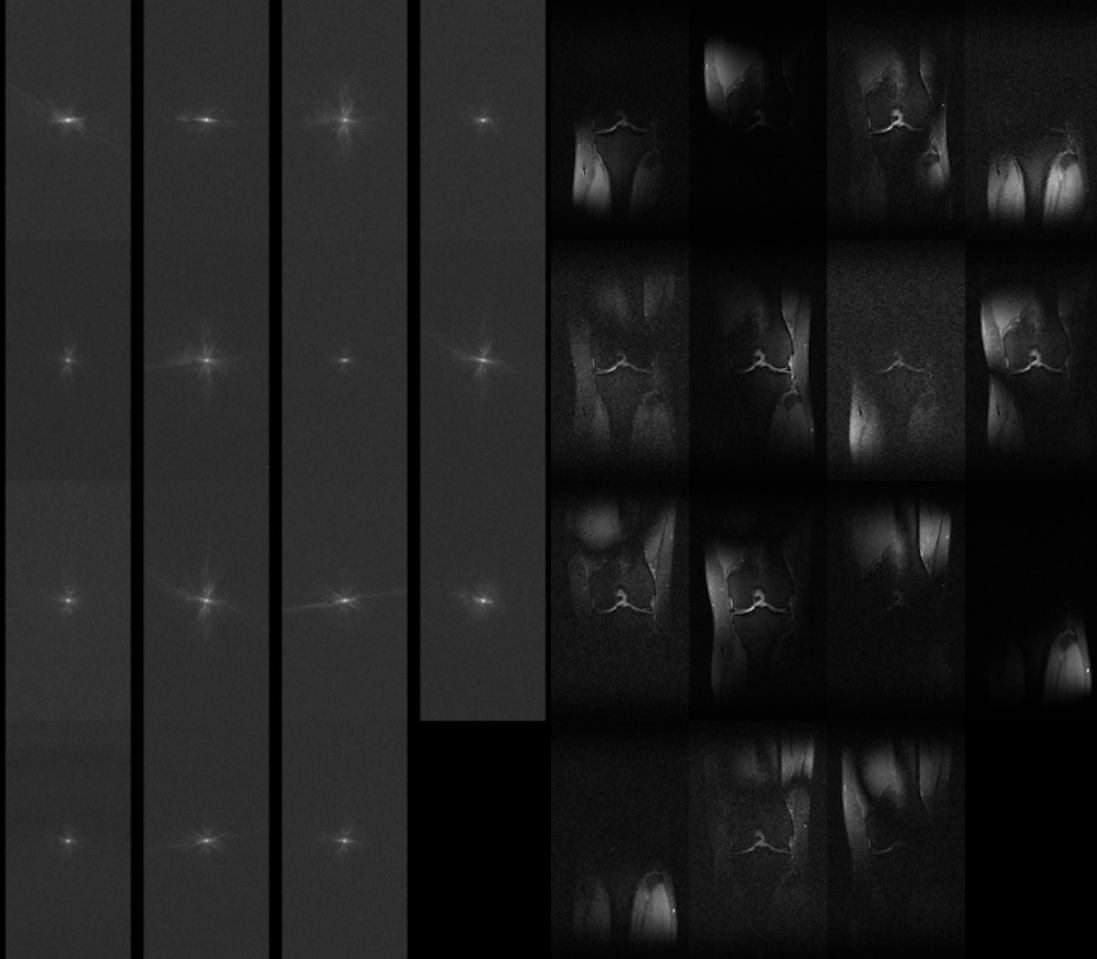
\includegraphics[width=150mm,scale=0.7]{kspace_coil.png}
    \caption{(a) FastMRI K-space data from 15 coils    (b) FastMRI individual fully sampled coil spatial images~\cite{zbontar_fastmri_2019, knoll_fastmri_2020}.}\label{visina8}
\end{figure}

\subsection{Sampling}

The time required to acquire all the measurements responses from every single atom in a subject would be extremely high and problematic to every one involved (pacients, doctors and clinics).
The way machines can do faster \ac{MRI} is by performing \textit{undersampling}, also referred as subsampling and sampling, when scanning the subject.

Undersampling is performed by giving the machine a known prescribed path in which it will extract measurements from the multidimensional k-space representation.
This allows machines to collect only a fraction of data measurements needed for image reconstruction hence speeding up the data acquisition process without critical quality loss.

There are some undersampling patterns to use and each has its benefits depending on several parameters, such as: the subject's region extraction, algorithm used for reconstruction, acquisition time.

In the figure below we can see some of the most used patterns.
In this research, we will focus mostly on the cartesian undersampling method, as that is the one used in the FastMRI dataset~\cite{zbontar_fastmri_2019, knoll_fastmri_2020}, which we will use for our experiments.

\begin{figure}[H]
    \centering
    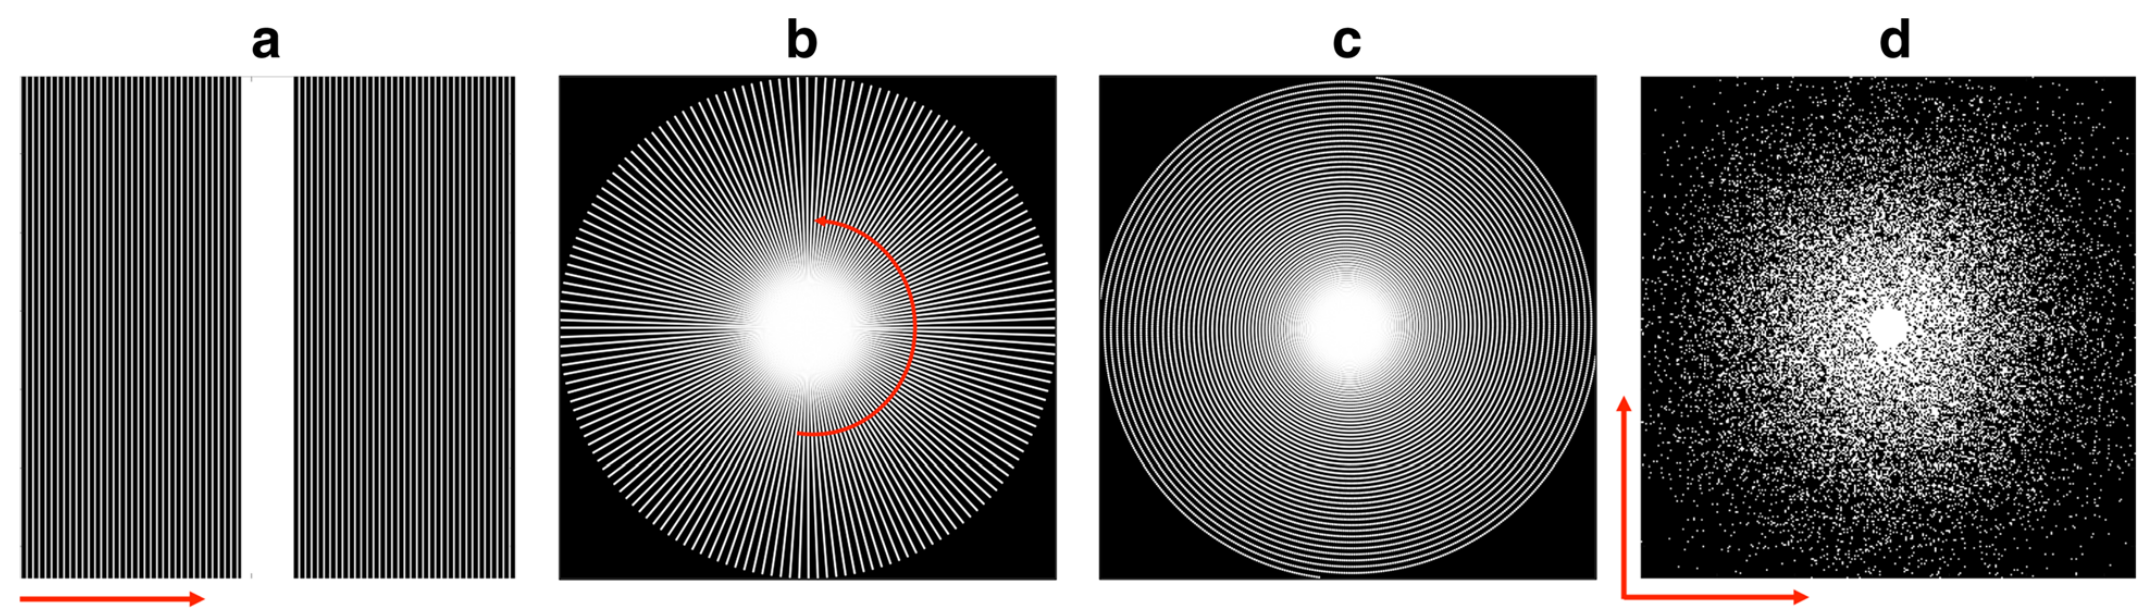
\includegraphics[width=150mm,scale=0.7]{sampling_trajectories}
    \caption{Under-sampling patterns. \textbf{(a) Cartesian undersampling}, \textbf{(b) radial undersampling}, \textbf{(c) spiral undersampling}, \textbf{(d) isolated samples in the k-space, according to the realisation of a random process}~\cite{ye_compressed_2019}.}\label{visina8}
\end{figure}


\section{Compressed Sensing}

\ac{CS} is an extremely powerful algorithm that was introduced in 2004 proposing a novel technique for the acquisition of signals of sparse or compressible nature.
\ac{CS} has disrupted the signal processing field as it has broken the \textit{Shannon's theorem}: the sampling signal rate must be at least twice the maximum frequency present in the signal (Nyquist rate).
\ac{CS} has been proven to sample the signal at a much lower rate than the Nyquist sampling rate.
In MRI, when \textit{k-space} is undersampled, the Nyquist criterion is violated~\cite{lustig_sparse_2007}.

The idea was inpired from questioning the necessity of extracting large portions of samples when much of these samples are discarded, exposing the inefficiency of trying to gather all signal.

%TODO fix quotation
\blockquote{Why go to so much effort to acquire all the data when most of what we get will be thrown away?
Can we not just directly measure the part that will not
end up being thrown away?~\cite{donoho_compressed_2006}}


\ac{CS} tackles the necessity to reconstruct signals with

\ac{CS} parts from the principle that if given $x$, a digital image or signal has a sparse representation in an orthonormal basis (e.g.wavelet, Fourier), then the $N$ most important coeffiecients in that expasion allow reconstruction with $l_2$ error $O(N^{1/2-1/p})$~\cite{donoho_compressed_2006}.


\section{Artificial Neural Networks}

\subsection{Biological Inspirations}

\ac{ANN}s, as the name suggests, have been (loosely) inpired by biological neural networks (brains) from animals.
The concept of using many layers of vector-valued representation is drawn from neuroscience.
The choice of the functions $f^{(i)}(x)$ used to compute these representations is also loosely guided by neuroscientific observations about the functions that biological neurons compute~\cite{goodfellow_deep_2016}.
Another trait they share is that just like the human brain can be trained to pass forward only meaningful signals to achieve larger goals of the brain, the neurons on a neural network can be trained to pass along only useful signal~\cite{patterson_deep_2017}.

\subsection{Neuron}

The most basic unit in \ac{ANN}s is the \textit{artificial neuron}.
These artificial neurons that are modeled mirroring the biological neurons behaviour as both of them are stimulated by inputs.
Each artificial neuron play an analogous role to a neuron carrying some information they receive to other artificial neurons in the \ac{ANN}.
Artificial neurons take in inputs $x_1, x_2,\ldots, x_n$, each and multiply them by their respective weights $w_1, w_2,\ldots, w_n$.
Then these weighted inputs are summed together producing the \textit{logit} of the artificial neuron, $z = \sum^n_{i=0} w_i x_i + b$, with $b$ being a constant number added called \textit{bias}.
After this, the logit is passed to a function $f$ in order to generate the value $y = f(z)$.

\begin{figure}[H]
    \centering
    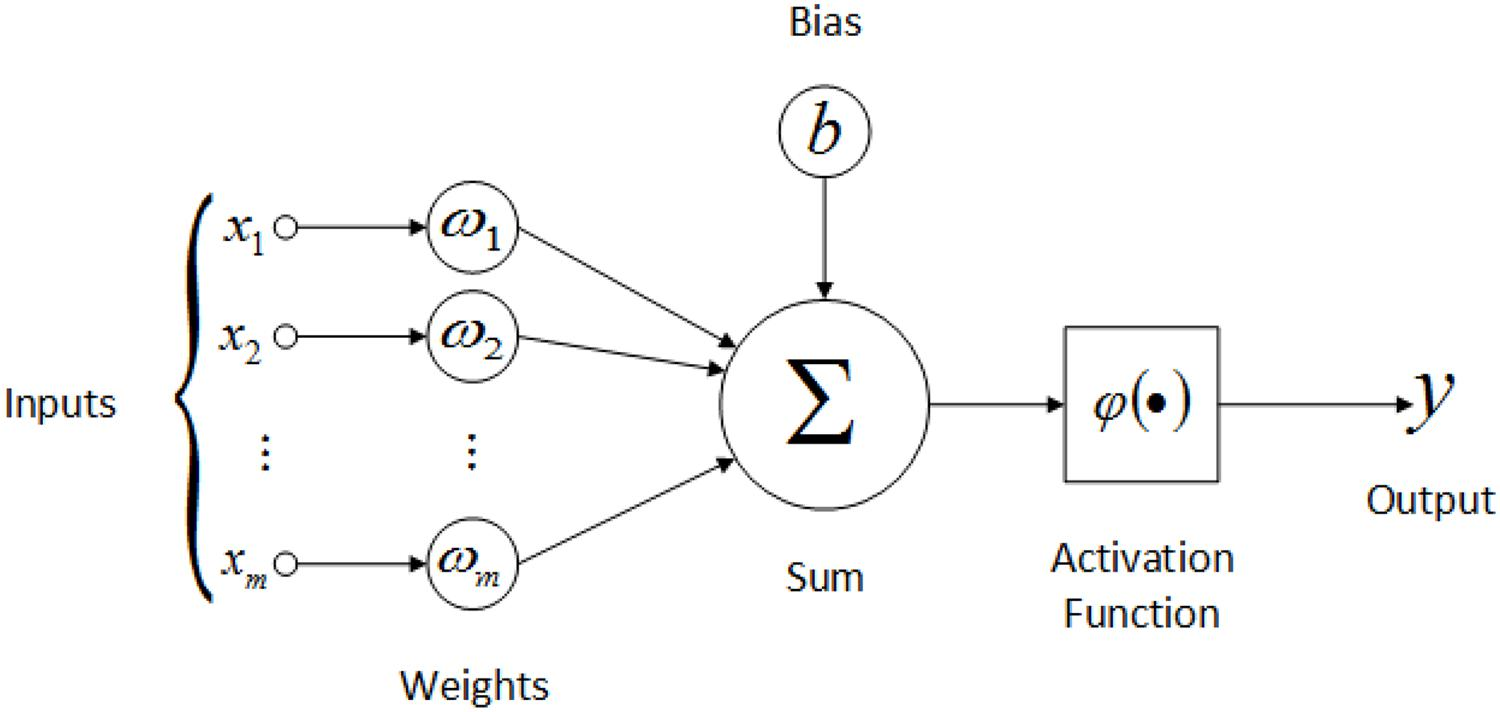
\includegraphics[width=150mm,scale=0.7]{neuron}
    \caption{Schematic of an Artificial Neuron.~\cite{quddus_machine_2018}}\label{visina8}
\end{figure}

\subsection{Multilayer Perceptron}

\ac{DFN} or \ac{MLP}s are a type of \ac{ANN} very commonly used.
It is the foundation to many famous architectures like \ac{CNN}s.
\ac{DFN}s have an input layer followed by one or many hidden layers and a single output layer.
Each layer is fully connected to the adjacent layer.

% TODO check quotation
\ac{MLP}s are computational models that flow information through the function that evaluates $x$.
The goal is to approximate some function $f*$, for instance, for a classifier, $y = f * (x)$ maps an input $x$ to a category $y$.
The feedforward defines a mapping $y = f(x;\theta)$ and learns the value of the parameters $\theta$ that result in the best function approximation~\cite{goodfellow_deep_2016}.

The behaviour of an \ac{ANN} is shaped by its architecture, which describes the number of units it should have and how these units connect to each other and how complex the model is.
Often adding too much complexity to the network will lead to overfitting the training set, which occurs when the model shapes the training data too preciselly and cannot generalise new data fed.

% TODO check plagi
Most \ac{ANN}s are organized into rows of neurons called layers.
These layers are arranged in a chain-like structure, with each layer being a function of the layer before it.
These layers' goal is to extract \textit{representations} out of the data fed and generalize what is meaningful towards minimizing the error rate.
This architecture scheme is represented by the following equation:

\begin{gather*}
    h^{(i)} = g^{(i)} (W^{(i)T}x + b^{(i)})
\end{gather*}

Where i is the layer index

\begin{figure}[H]
    \centering
    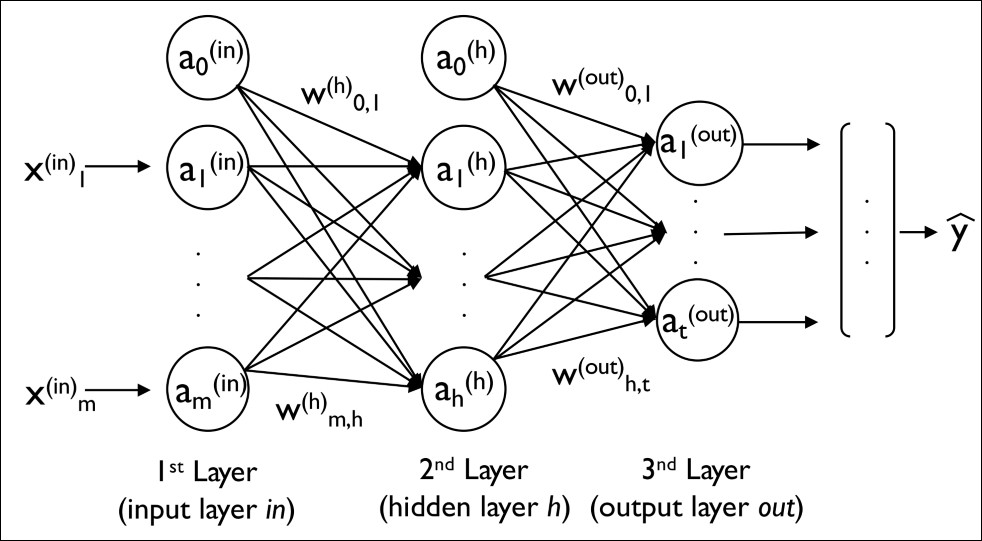
\includegraphics[width=0.7\textwidth]{mlp_architecture}
    \caption{\ac{ANN} Architecture Sample.}\label{visina8}
\end{figure}

\subsection{Activation Functions}

Activation functions are a scalar-to-scalar function used to propagate the output of one layer's neurons forward to the next layer.
There are several types of activation functions for different purposes and network architectures.

The \ac{DCGAN} architecture used in my MNIST experiment is built using \ac{ReLU} activations in the generator network and a \textit{tanh} in the output layer.
The discriminator network uses LeakyReLU activations for all layers and a \textit{sigmoid} function for the output layer.
LeakyReLU activation functions~\cite{maas_rectier_nodate, empirical_relu_cnn} have been proven to work well for higher resolution modeling~\cite{radford_unsupervised_2016} in contrast to the usage of maxout activation functions that were first proposed in the original \ac{GAN} paper~\cite{goodfellow_generative_2014}.

\begin{table}[H]
    \centering
    \begin{tabular}{l|c|c|cc|}
      \toprule
      Name & Function & Derivative & \\
      \midrule
      \hline
      Sigmoid & $\phi(x) = \dfrac{1}{1+e^{-x}}$ &  $\phi'(x) = \phi(x)(1-\phi(x))$\\[3ex]
      TanH    & $\phi(x) = \dfrac{2}{1+e^{-2x}} - 1$ & $\phi'(x) = 1-\phi(x)^2$ \\[3ex]
      ReLU    & $\phi(x) = \begin{cases}
                           0 & x \leq 0 \\
                           x & x > 0
                         \end{cases} $
                         & $\phi'(x) = \begin{cases}
                                           0 & x \leq 0 \\
                                           1 & x > 0
                                         \end{cases} $ \\[4ex]
      Leaky ReLU & $\phi(x) = \begin{cases}
                           \alpha x & x \leq 0 \\
                           x & x > 0
                         \end{cases} $
                         & $\phi'(x) = \begin{cases}
                                           \alpha & x \leq 0 \\
                                           1 & x > 0
                                         \end{cases} $ \\
      \bottomrule
    \end{tabular}
    \caption{Activation functions and their derivatives.}
    \label{tab:activation-functions}
\end{table}

Some of the most used and also required activation functions in the use of \ac{GAN}s and other widely used neural networks are described below.

\subsubsection{\ac{ReLU}}

The \ac{ReLU}~\cite{hahnloser_digital_2000} transform activates a node only if the input is above a certain threshold having a linear relationship with the dependent variable and outputs zero for every input below zero.

\begin{figure}[H]
    \centering
    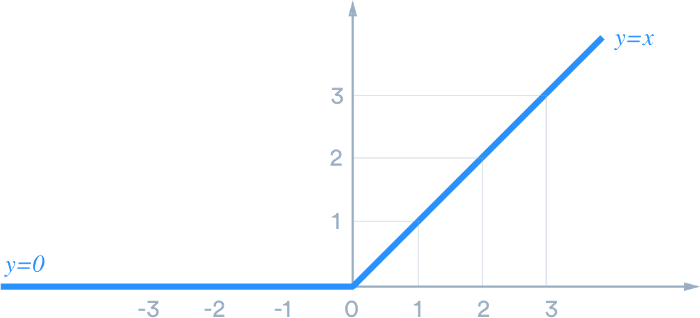
\includegraphics[width=0.6\textwidth]{relu}
    \caption{\ac{ReLU} activation function}\label{visina8}
\end{figure}

\subsubsection{Leaky ReLU}

\ac{ReLU} activation functions have the ``dying ReLU'' problem, where a ReLU neuron is stuck in the negative side and always outputs 0~\cite{trottier_2017, deep_learning_relu}.
This happens when the slope of \ac{ReLU} in the negative range is also 0, once a neuron gets negative, it is unlikely for it to recover.
These ``dead'' neurons are not playing any role in discriminating the input and are essentially useless.

To mitigate this issue within \ac{ReLU}s, LeakyReLUs are a strategy that opposed to having the function being zero when $x < 0$, it has instead a small negative slope (most times with $\alpha = 0.01$).

\begin{figure}[H]
    \centering
    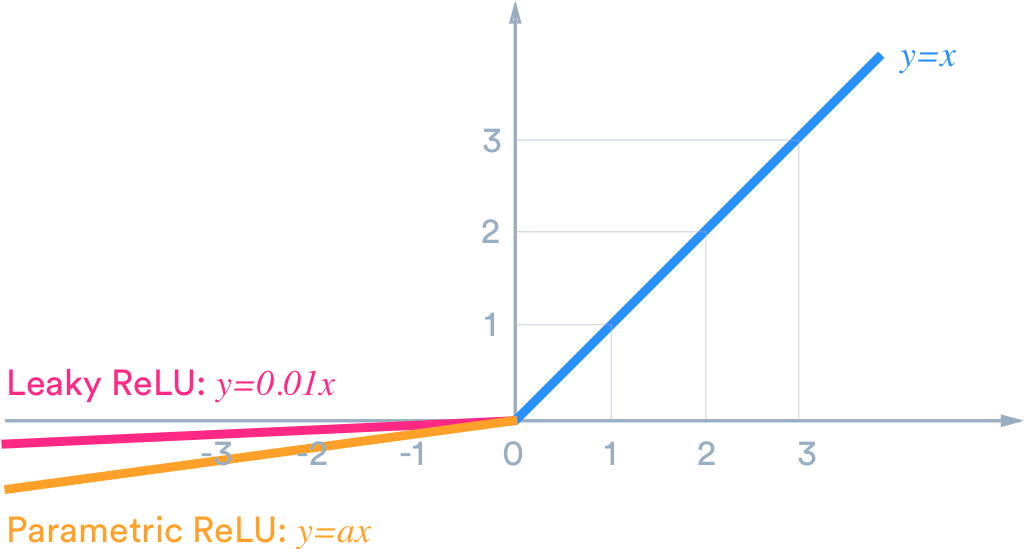
\includegraphics[width=0.6\textwidth]{leaky_relu}
    \caption{Leaky \ac{ReLU} activation function}\label{visina8}
\end{figure}

\subsubsection{Tanh}

Tanh is a hyperbolic trigonometric function that deals more easily with negative numbers~\cite{patterson_deep_2017}. Unlike the Sigmoid function, tanh ranges from -1 to 1.

\begin{figure}[H]
    \centering
    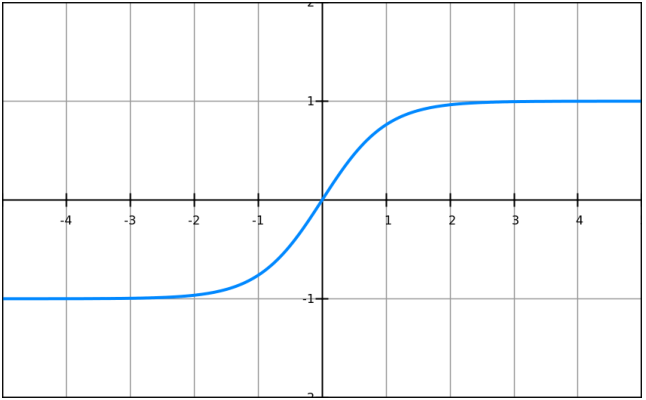
\includegraphics[width=0.6\textwidth]{tanh}
    \caption{\textit{Tanh} activation function. Source:~\cite{patterson_deep_2017}}\label{visina8}
\end{figure}

\subsubsection{Sigmoid}

Sigmoids can reduce extreme values or outliers in data without removing them, framing the input from 0 to 1 and most outputs will be close to either 0 or 1.

\begin{figure}[H]
    \centering
    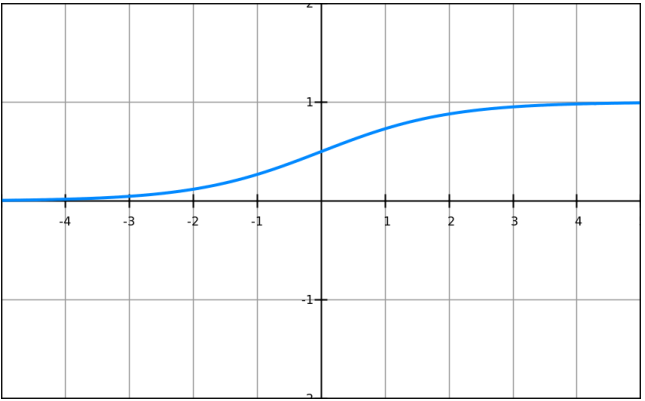
\includegraphics[width=0.6\textwidth]{sigmoid}
    \caption{Sigmoid activation function. Source:~\cite{patterson_deep_2017}}\label{visina8}
\end{figure}

\subsection{Loss Functions}

Loss functions are used to determine how a neural network is perfoming on the given data.
A metric is calculated based on the error observed in the network's predictions and the model then tries to minimize this error in a optimization problem fashion.

Some of the most commonly used functions are described in the table below.

\begin{table}[H]
    \centering
    \begin{tabular}{|lccc}
      \midrule
        Mean squared error & MSE &= &$\displaystyle\frac{1}{n}\sum_{t=1}^{n}e_t^2$   \\
        \hline
        Root mean squared error & RMSE &= &$\displaystyle\sqrt{\frac{1}{n}\sum_{t=1}^{n}e_t^2}$ \\
        \hline
        Mean absolute error & MAE &= &$\displaystyle\frac{1}{n}\sum_{t=1}^{n}|e_t|$ \\
        \hline
        Mean absolute percentage error & MAPE &= &$\displaystyle\frac{100\%}{n}\sum_{t=1}^{n}\left |\frac{e_t}{y_t}\right|$\\
    \end{tabular}
    \caption{Loss functions and their formulas.}
    \label{tab:loss-functions}
\end{table}

In the case of generative networks, the original \ac{GAN} paper presents a loss function called \textit{minmax}~\cite{goodfellow_generative_2014}, that is described as.

\begin{equation}
    min_Gmax_DV(D,G)= E_{x\sim P_{data}(x)}[logD(x)]+E_{z\sim pz(z)}[log(1 - D(G(z)))]
\end{equation}

Where $x$ is the input data representing an image, $D(x)$ is the discriminator network, $G(x)$ is the generator function and $z$ represents the latent vector that is mapped to data-space by $G$.
Hence, the scalar probability that the output of the generator $G$ is a real image is given by $D(G(z))$~\cite{goodfellow_generative_2014}.


\subsection{Backpropagation}

%TODO

In multi-layer networks, the gradient of a composition function is computed using the backpropagation~\cite{backpropagation_1986}, that computes the error derivatives with respect to a single training example.

\subsection{Stochastic Gradient Descent}

\ac{SGD} 
%TODO

Most deep learning models are powered by the \ac{SGD}, which is an extension of the gradient descent algorithm.

\begin{figure}[H]
    \centering
    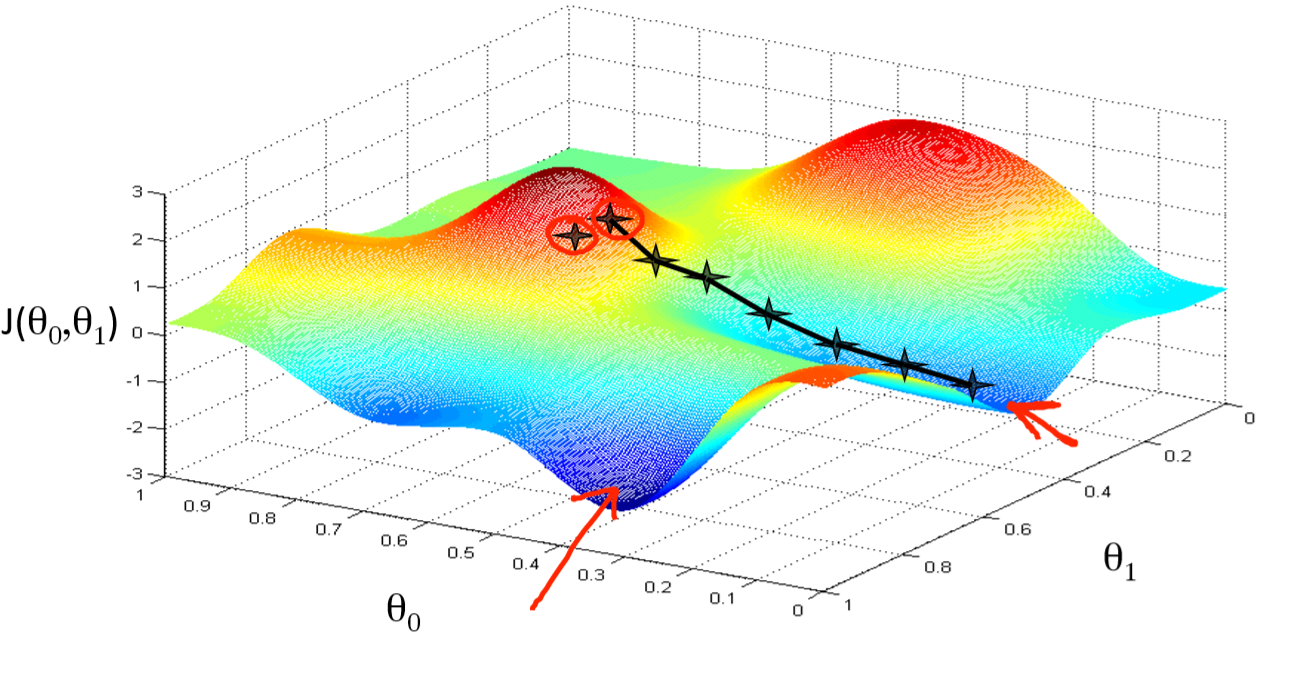
\includegraphics[width=0.6\textwidth]{gradient_descent}
    \caption{Gradient Descent example visualization.}\label{visina8}
\end{figure}

\section{Generative Adversarial Networks}

\ac{GAN}s are a machine learning strategy proposed in 2014 by Ian Goodfellow~\cite{goodfellow_generative_2014} that consists of two simultaneously trained models: the \textit{Generator} $G(x)$ and the \textit{Discriminator} $D(x)$.
The generator has the role to generate fake data whilst the discriminator is trained to discern wheter the given input is real or fake.

In essence, the generator takes a vector of random numbers $(z)$ as input and outputs a fake example that strives to look as close as possible to the training data pattern.
The discriminator takes an image $(x)$ as input from two sources: real examples from the training set and fake examples generated by the generator network, then the discriminator outputs a scalar probability that the image is real~\cite{langr_gans_2019}.

\ac{GAN}s play a minimax two-player game in which $D$ tries to maximize the probability to correctly classify real and fake samples ($\log D(x)$), whilst $G$ tries to minimize the chance that $D$ will correctly predict its generated outputs are fake ($\log (1-D(G(x)))$).

Ideally, this minimax game would resolve to a solution with $pg=p_{data}$, where the discriminator is incapable of distinguishing real from fake inputs. 
However, \ac{GAN}s are still a novel neural network approach with its convergence theory is still being highly researched and hardly reaching this point in reality~\cite{goodfellow_generative_2014}.

\begin{figure}[H]
    \centering
    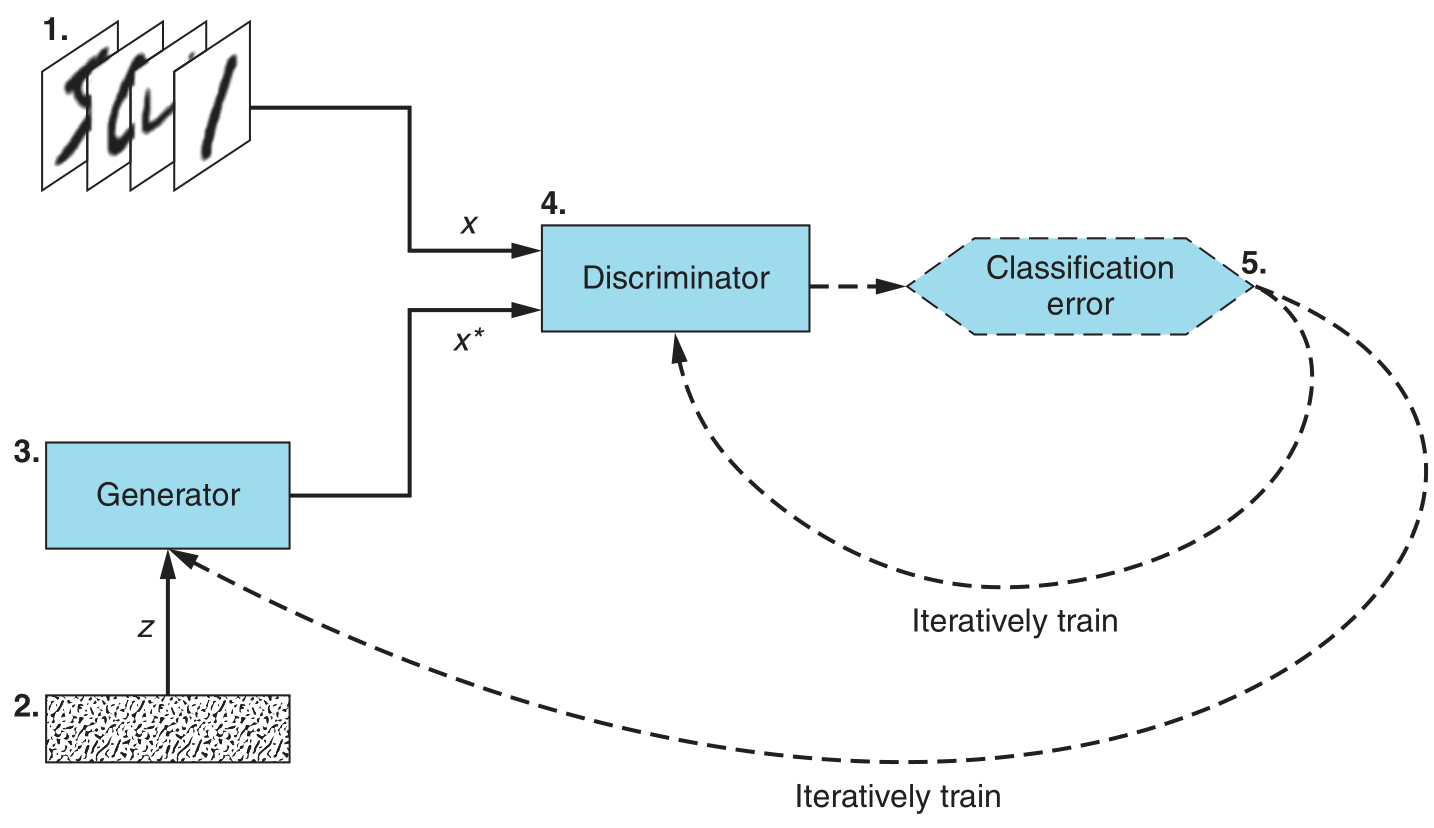
\includegraphics[width=\textwidth]{gan_schema}
    \caption{\ac{GAN} training diagram. Source:~\cite{langr_gans_2019}}\label{visina8}
\end{figure}

%---}}}

% |--- Methodology ---|----------------------{{{
\chapter{Methodology}

\section{1-D Direct vs Indirect L1-Minimization}

L1-minimization admits both direct and indirect approaches, in which there is the accuracy x resources trade-off.
The direct method often produces a higher quality reconstruction but is very memory consuming, whilst the indirect method loses a little bit of quality, but requires much less memory to compute the equations system.

To visualize this trade-off, I have created 200 random 1-D arrays ranging values from the standard normal distribution and have taken 10\% of data points randomly to reconstruct the whole signal using different $L$ sizes.

The $L$ variable denotes the %TODO
The figure below displays the first 10 signals created.

\begin{figure}[H]
    \centering
    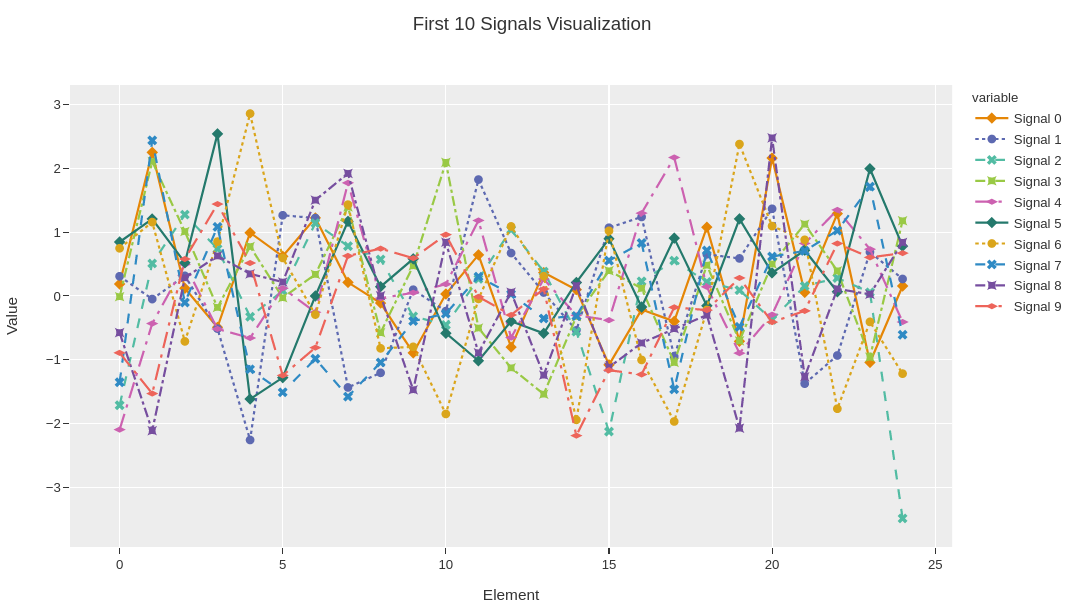
\includegraphics[width=\textwidth]{1d_signal_plot}
    \caption{First 10 random 1-D signals}\label{visina8}
\end{figure}

\section{Phantom Compressed Sensing Reconstruction with Pre Filtered Signal}

To test the method of applying pre-filtering to the input signals in the k-space, I have conducted an experiment with the well-known Shepp-Logan phantom~\cite{shepp_fourier_1974} to evaluate how the usage of sparsifying filters impact the total-variation minimization~\cite{miosso_compressive_2009-1}.

\subsection{Subsampling}

I then created an phantom image with dimension of $256\times256$, hence 65536 data points, using the phantominator python module.
Then, I simulated an undersampled phantom image by applying the spiral undersampling pattern achieving approximately 30.95\% of data points from the fourier space which resulted in a matrix with 20285 non zero elements.

\begin{figure}[H]
  \centering
  \begin{minipage}[b]{0.4\textwidth}
    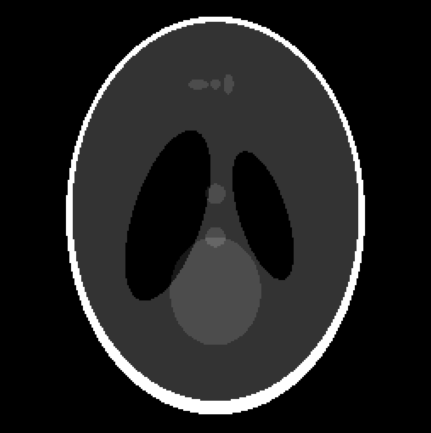
\includegraphics[width=\textwidth]{phantom_shepplogan.png}
    \caption{Shepp-Logan phantom reference image.}
  \end{minipage}
  \begin{minipage}[b]{0.4\textwidth}
    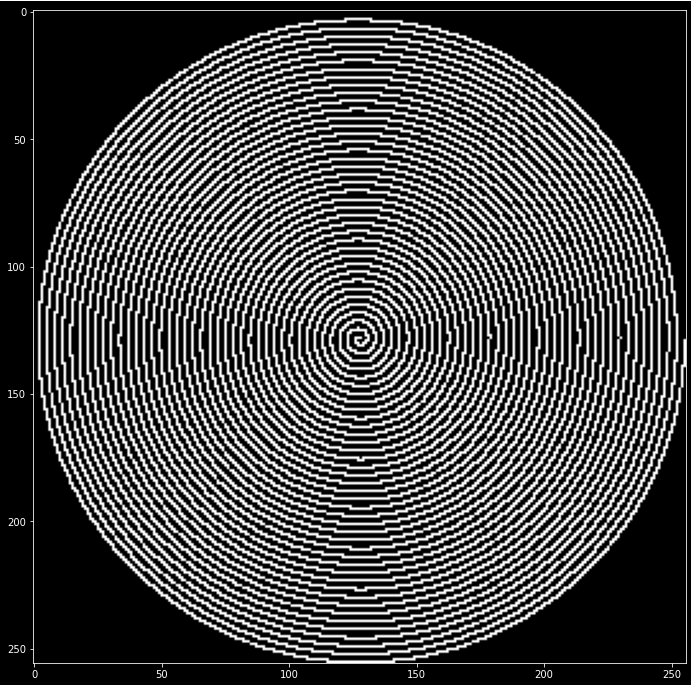
\includegraphics[width=\textwidth]{spiral_phantom_experiment.png}
    \caption{Spiral undersampling method with 30.95\% data points.}
  \end{minipage}
\end{figure}

\subsection{Pre-filtering sparsifying transform}

For the pre-filtering step, three filters are used to increase sparsity in the signal to be reconstructed.
The filters are all $2\times2$ matrices and increase the sparsity in the signal from different perspectives, using more filters leverages the ability to sparsify the signal.
The filtered images are then composed to one single image containing the highest gain each filter could provide given a single pixel in the image~\cite{miosso_compressive_2009-1}.
The different filters used can be better seeing in the figure below.

\begin{figure}[H]
  \centering
  \begin{minipage}[b]{0.3\textwidth}
      
\includegraphics[width=\textwidth]{filter1.png}
      \caption{2-D High pass horizontal filter.}
  \end{minipage}
  \begin{minipage}[b]{0.3\textwidth}
      
\includegraphics[width=\textwidth]{filter2.png}
      \caption{2-D High pass vertical filter.}
  \end{minipage}
  \begin{minipage}[b]{0.3\textwidth}
      
\includegraphics[width=\textwidth]{filter3.png}
      \caption{2-D High pass diagonal filter.}
  \end{minipage}
\end{figure}

The pre-filtering method is evaluated against the zero-fill reconstruction method (used as a dummy baseline) and a L1-minimization method without pre-filtering with the very same parameters used in the pre-filtering L1-minimization.


\section{Preliminary Tests with Generative Adversarial Networks}

In order to test the usage of \ac{GAN}s for data generation and in the future use it along with \textit{prior information} for \ac{CS} systems, I have developed a \ac{GAN} capable of generating handwritten digits from 0 to 9 using the notable MNIST dataset.
The MNIST dataset contains 60,000 examples for training and 10,000 examples for testing.
The digits have been size-normalized and centered in a fixed-size image ($28\times28$ pixels) with values from 0 to 9.
For simplicity, each image has been flattened and converted into a 1-dimensional numpy array of 784 features ($28\times28$).

The idea is to test if the neural network can output liable digits that look both readable (to the extent in which the MNIST dataset is) and also like it has been made by a human, just like the dataset itself.

Each MNIST image contains a $28\times28$ black and white image, like the following:

\begin{figure}[H]
    \centering
    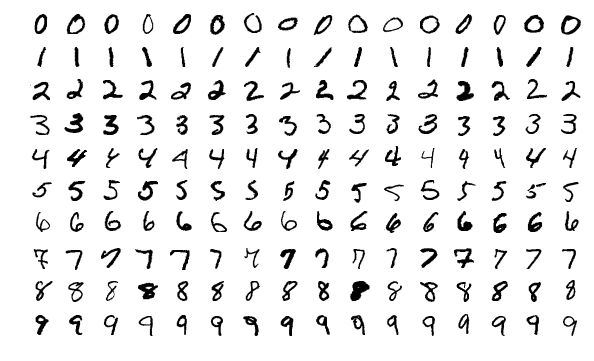
\includegraphics[scale=0.7]{mnist_sample}
    \caption{Sample of digits from MNIST}\label{visina8}
\end{figure}

A \ac{DCGAN} was used for the experiment. A \ac{DCGAN} is an extension of the \ac{GAN}, except that it explicitly uses convolutional and convolutional-transpose layers in the discriminator and generator networks, respectively~\cite{radford_unsupervised_2016}.

\subsection{Data Transformation}

Each input image used by the \textit{dataloader} went through a computer-vision pre-processing step that include:

\begin{itemize}
    \item Grayscale transform: convert the image to greyscale. When loaded, the MNIST digits are in RGB format with three channels. Greyscale reduces these three to one.
    \item ToTensor: convert the image to a PyTorch Tensor, with dimensions (channels, height, width). This also rescales the pixel values, from integers between 0 and 255 to floats between 0.0 and 1.0.
    \item Normalize: scale and translate the pixel values from the range 0.0, 1.0 to -1.0, 1.0. The first argument is \( \mu \) and the second argument is \( \sigma \), and the function applied to each pixel is:
    \begin{equation}
        \rho \leftarrow \frac{(\rho - \mu)}{\sigma}
    \end{equation}
\end{itemize}

\subsection{Generator Network Architecture}

The generator network architecture is implemented using PyTorch as:

\begin{itemize}
    \item A linear \textit{fully-conected} module (or layer) to map the latent space to a $7 * 7 * 256 = 12544$ dimensional space that will later be undersampled several times until we reach $1\times28\times28$.
    \item An optional 1-dimensional batch normalization module
    \item A leaky ReLU module.
    \item A 2-dimensional convolutional layer with $padding=2$, $stride=1$ and $5\times5$ kernel (or filter).
    \item Two 2-dimensional transposed convolutional layers with $padding=1$, $stride=2$ and $4\times4$ kernel.
    \item Two optional 2-dimensional batch normalization modules after each 2-dimensional transposed convolutional layer.
    \item A \textit{Tanh} activation function, rescaling the images to a $[-1, 1]$ range.
\end{itemize}

\begin{figure}[H]
    \centering
    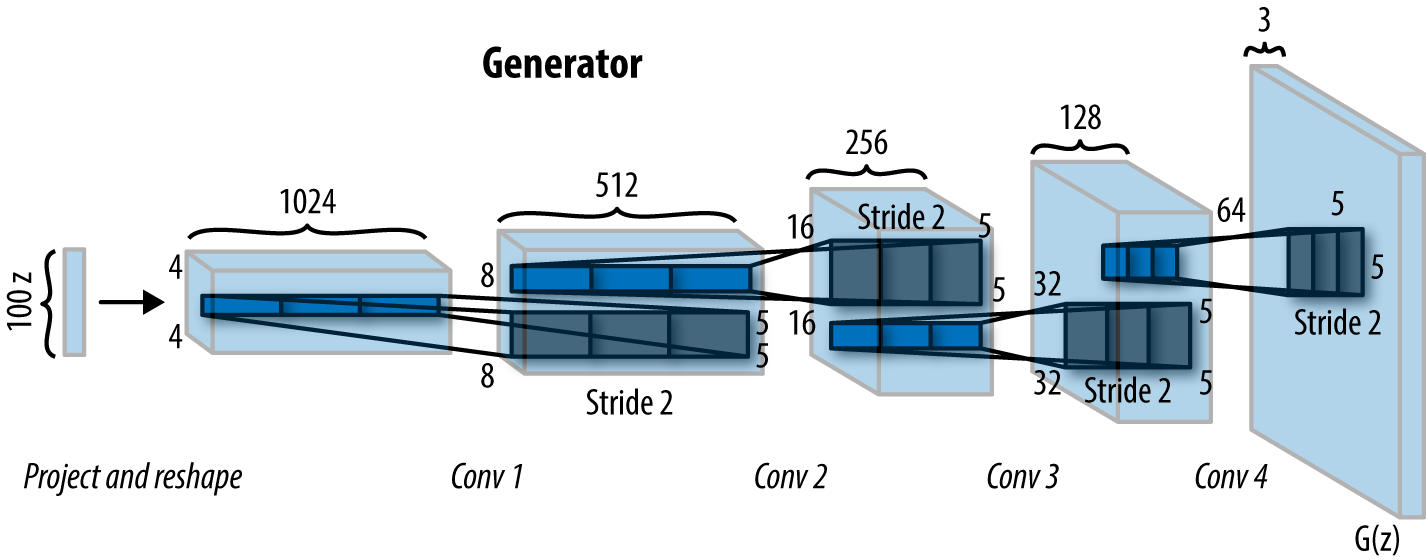
\includegraphics[width=\textwidth]{generator}
    \caption{Generator network architecture of a 3-D image. Source:~\cite{radford_unsupervised_2016, oreilly_gan}}\label{visina8}
\end{figure}

The latent space (random signal) input goes through each layer being upscaled until it reaches the target image dimension $28\times28$ and then fed into the discriminator network.

\subsection{Discriminator Network Architecture}

The discriminator is a \ac{CNN}-based image binary classifier network that takes an image as input and outputs a scalar probability that the given image is real or generated.
The architecture is quite similar to the Generator network, except backwards.
Here, the discriminator takes a $1\times28\times28$ input image, processes it through a series of convolutions, batch normalizations, and LeakyReLU layers, and outputs the final probability through a Sigmoid activation function.

\begin{figure}[H]
    \centering
    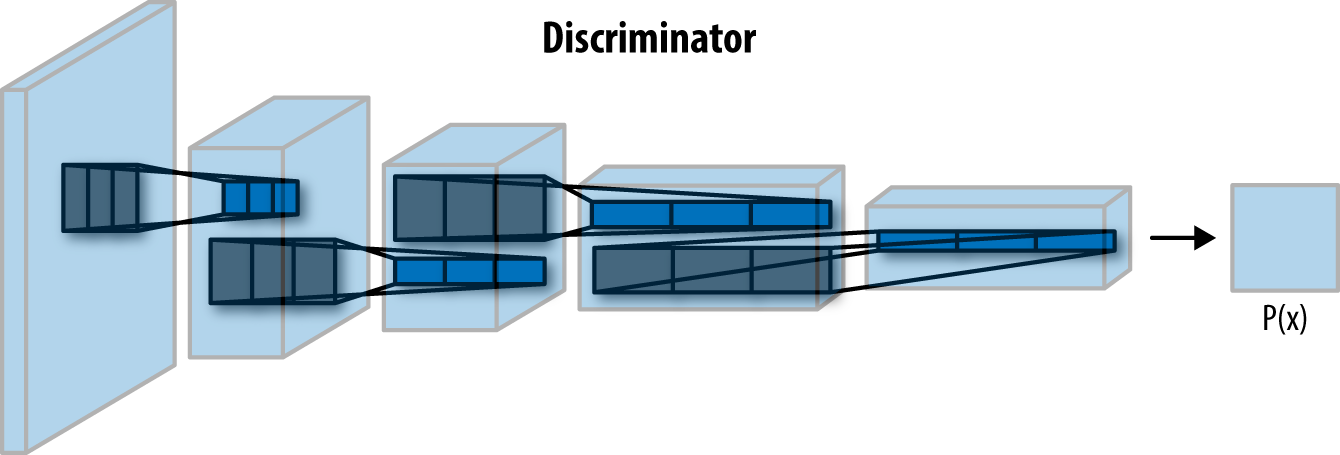
\includegraphics[width=\textwidth]{discriminator}
    \caption{Discriminator network architecture of a 3-D image. Source:~\cite{radford_unsupervised_2016, oreilly_gan}}\label{visina8}
\end{figure}
%---}}}

% |--- Results ---|----------------------{{{
\chapter{Preliminary Results}

\section{1-D Compressed Sensing Reconstruction}

The quality over resources demanded trade-off really starts making a big difference with L size around 200 samples, which is close to 80\% of the data present in the signal to be reconstructed.
This demonstrates that there is no big prejudice in using indirect reconstrution method
for very undersampled signals (close to 10\% of the data) such as the ones used in \ac{MRI}

\begin{figure}[H]
    \centering
    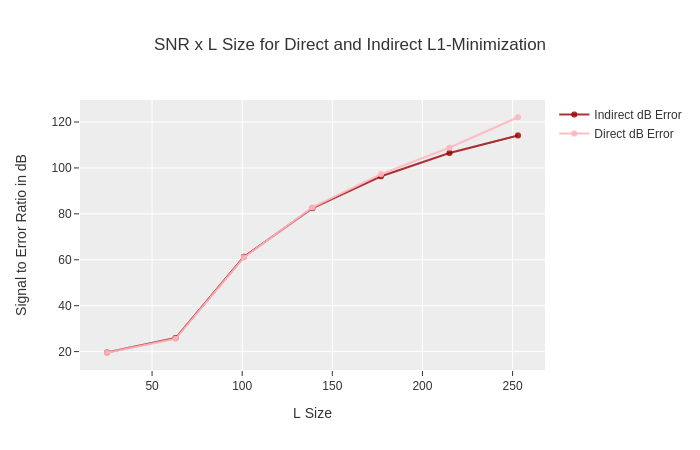
\includegraphics[scale=0.7]{snr_lsize_experiment}
    \caption{\ac{SNR} x \textit{L} size for direct and indirect L1-minimization for 200 random 1d signals}\label{visina8}
\end{figure}

\section{Compressed Sensing Reconstruction with Pre Filtered Signal}

The results in the experiment shows a huge gain of resolution in the pre-filtering method reconstructed image compared to the L1-minimization alone.

The zero-filled reconstruction (dummy baseline) was unable to reconstruct a high fidelity image and performed very poorly in the PSNR and SNR metrics.
The L1-minimization compressed sensing approach reconstructed the image with some noticeable noise artifacts, yet much better than the zero-filling approach.
Finally, the L1-minimization along the usage of sparsifying pre-filtering delivered a great looking image without eye-catching artifacts and also increased the metrics hugely.

\begin{figure}[H]
  \centering
  \begin{minipage}[t]{0.22\textwidth}
    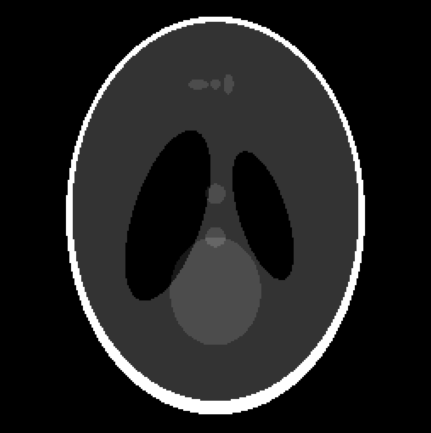
\includegraphics[width=\textwidth]{phantom_shepplogan.png}
    \caption{Phantom reference image}
  \end{minipage}
  \begin{minipage}[t]{0.22\textwidth}
    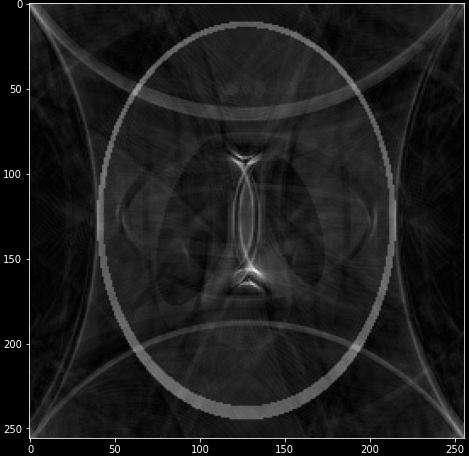
\includegraphics[width=\textwidth]{recon_zero_fill.png}
    \caption{Phantom zero-filled reconstruction}
  \end{minipage}
  \begin{minipage}[t]{0.22\textwidth}
    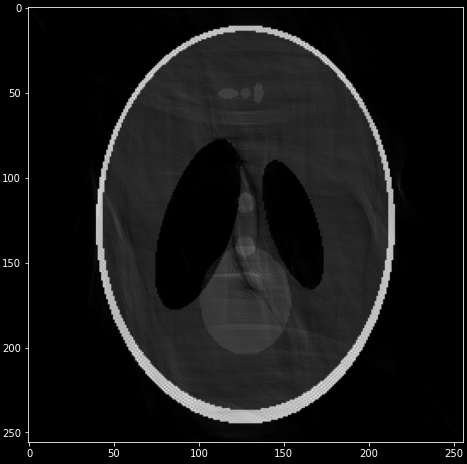
\includegraphics[width=\textwidth]{recon_l1.png}
    \caption{Phantom L1-minimization reconstruction}
  \end{minipage}
  \begin{minipage}[t]{0.22\textwidth}
    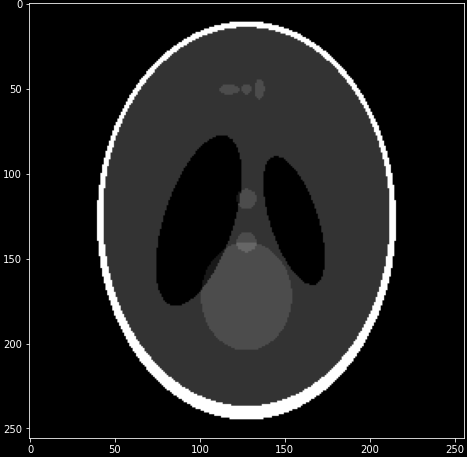
\includegraphics[width=\textwidth]{recon_prefilter.png}
    \caption{Phantom L1-minimization with pre-filtering reconstruction}
  \end{minipage}
\end{figure}

The usage of L1-minimization for certainly improves the \ac{MRI} reconstruction, but the metrics reinforce how adding the pre-filtering step to preprocess the image achieves incredibly higher scores in \ac{PSNR} and \ac{SNR}.

\begin{table}[h!]
  \begin{center}
    \begin{tabular}{l|llll}
                                        & \textbf{PSNR}  & \textbf{SSIM}   & \textbf{SNR}  & \textbf{MSE}     \\
      \hline
        \textbf{Zero-fill}                             & 22.41 & 0.36 & 4.22 & 0.02     \\
        \textbf{L1-minimization}                       & 38.76 & 0.96 & 20.57 & 5.3e-5   \\
        \textbf{Pre-filtering L1-minimization}         & 91.89 & 0.99 & 73.70 & 2.5e-9
    \end{tabular}
  \end{center}
  \caption{Phantom reconstruction metrics.}
  \label{tab:phantom-reconstruction}
\end{table}

\subsection{Brain Sagittal Reconstruction}

Another experiment done was using a reference sagittal head image of shape $(256 \times 256)$.
The same spiral undersampling pattern with 30.95\% data points used in the phantom experiment was used here for artificial undersampling.

This image poses a harder reconstruction challenge as it is filled with more details and more complex structures than the phantom.
That said, it is clear that the undersampling pattern and amount of data points has not been sufficient to reconstruct a high fidelity image in any scenario, but the L1-minimization with pre-filtering reconstruction looks like the winner again, reinforcing the idea that pre-filtering is a good pre-processing strategy.

\begin{figure}[H]
  \centering
  \begin{minipage}[t]{0.22\textwidth}
    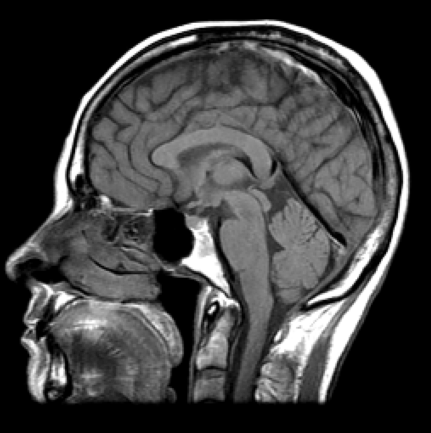
\includegraphics[width=\textwidth]{head}
    \caption{Sagittal head reference image}
  \end{minipage}
  \begin{minipage}[t]{0.22\textwidth}
    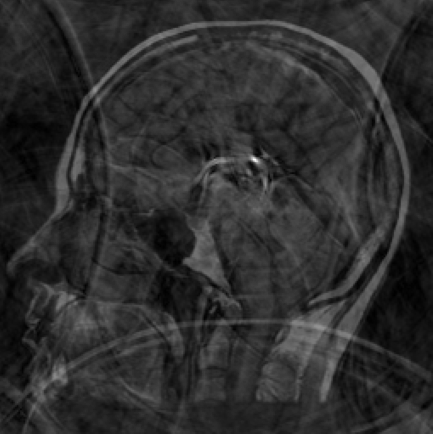
\includegraphics[width=\textwidth]{recon_head_zero_fill}
    \caption{Sagittal head zero-filled reconstruction}
  \end{minipage}
  \begin{minipage}[t]{0.22\textwidth}
    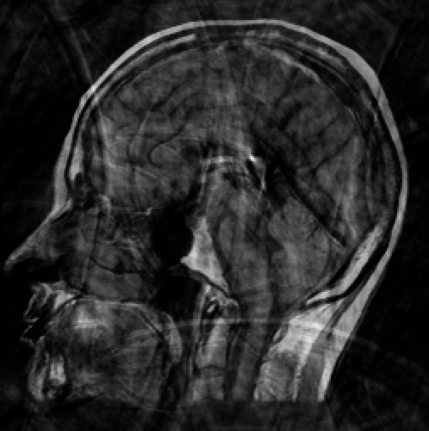
\includegraphics[width=\textwidth]{recon_head_l1}
    \caption{Sagittal head L1-minimization reconstruction}
  \end{minipage}
  \begin{minipage}[t]{0.22\textwidth}
    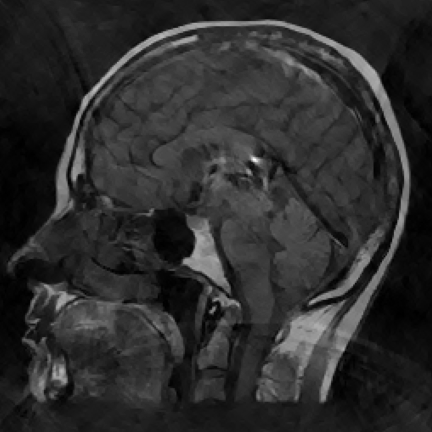
\includegraphics[width=\textwidth]{recon_head_prefilter}
    \caption{Sagittal head L1-minimization with pre-filtering reconstruction}
  \end{minipage}
\end{figure}

The metrics evaluated were not affected as much as they were for the phantom experiment, but they were mostly improved by the pre-filtering usage.

\begin{table}[h!]
  \begin{center}
    \begin{tabular}{l|llll}
                                        & \textbf{PSNR}  & \textbf{SSIM}   & \textbf{SNR}  & \textbf{MSE}     \\
      \hline
        \textbf{Zero-fill}                             & 17.68 & 0.32 & 5.52 & 2392.57 \\
        \textbf{L1-minimization}                       & 21.51 & 0.43 & 8.76 & 1134.88  \\
        \textbf{Pre-filtering L1-minimization}         & 21.03 & 0.45 & 8.97 & 1081.53
    \end{tabular}
  \end{center}
  \caption{Sagittal reconstruction metrics.}
  \label{tab:sagittal-reconstruction}
\end{table}

\subsection{Knee Singlecoil Reconstruction}

\begin{figure}[H]
  \centering
  \begin{minipage}[t]{0.22\textwidth}
    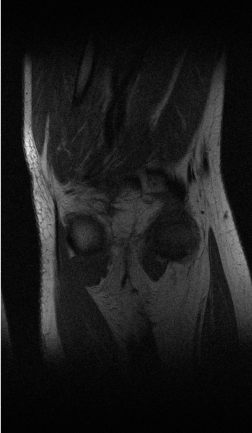
\includegraphics[width=\textwidth]{singlecoil_knee_fullysampled.png}
    \caption{Singlecoil knee reference image}
  \end{minipage}
  \begin{minipage}[t]{0.22\textwidth}
    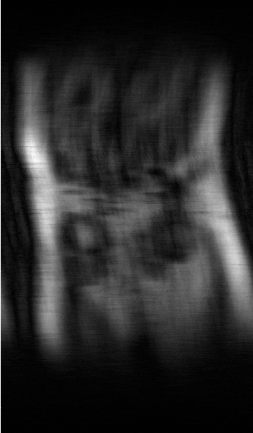
\includegraphics[width=\textwidth]{recon_zero_filled_knee.png}
    \caption{Knee zero-filled reconstruction}
  \end{minipage}
  \begin{minipage}[t]{0.22\textwidth}
    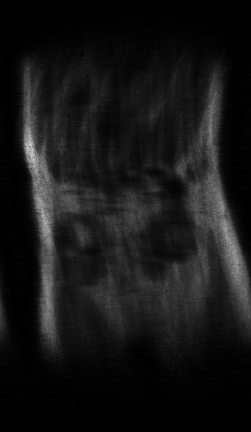
\includegraphics[width=\textwidth]{recon_singlecoil_knee.png}
    \caption{Knee L1-minimization reconstruction}
  \end{minipage}
  \begin{minipage}[t]{0.22\textwidth}
    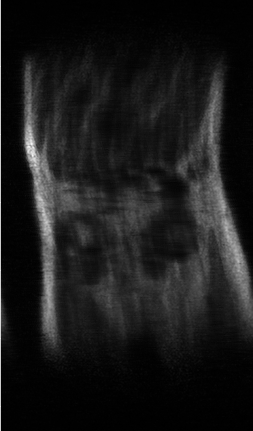
\includegraphics[width=\textwidth]{recon_prefiltering_singlecoil_knee.png}
    \caption{Knee L1-minimization with pre-filtering reconstruction}
  \end{minipage}
\end{figure}


\begin{table}[h!]
  \begin{center}
    \begin{tabular}{l|llll}
                                        & \textbf{PSNR}  & \textbf{SSIM}   & \textbf{SNR}  & \textbf{MSE}     \\
      \hline
        \textbf{Zero-fill}                             &  &  &  &  \\
        \textbf{L1-minimization}                       &  &  &  &   \\
        \textbf{Pre-filtering L1-minimization}         &  &  &  & 
    \end{tabular}
  \end{center}
  \caption{Singlecoil knee reconstruction metrics.}\label{tab:singlecoilknee-reconstruction}
\end{table}

\section{Preliminary Tests with Generative Adversarial Networks}


Both discriminator losses (fake and real) start very high and quickly decreases as the generator loss curve goes up in an invertly correlated manner.
This happens specially because the generator starts by tricking the discriminator network very easily as it is na�ve to determine if an image is real or generated.
Quickly the discriminator starts to detect how the data is disposed and manages to interpret the generated images are different from the training examples it is seeing.

This phenoma exposes how bad the generator is in the first epochs and how easily the discriminator can distinguish between created and real.
Then as the epochs go by and both networks get more sophisticated, the generator starts to get better at creating the desired signal style and makes the discriminator's loss get higher again as it is observed in the loss curves below.

\begin{figure}[H]
  \centering
  \begin{minipage}[t]{0.4\textwidth}
    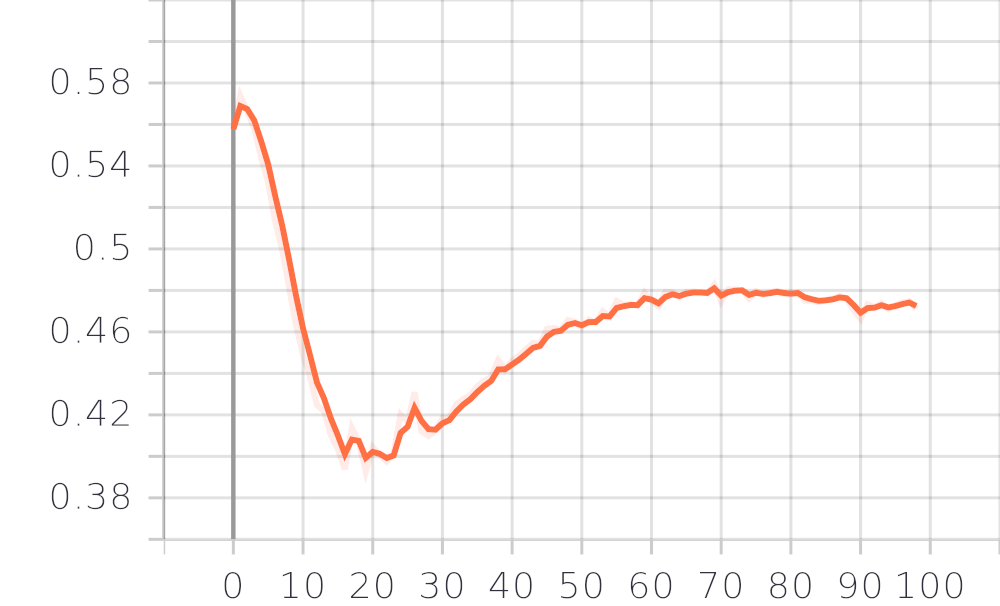
\includegraphics[width=\textwidth]{Discriminator_Loss_Fake}
    \caption{Discriminator fake loss over epochs}
  \end{minipage}
  \begin{minipage}[t]{0.4\textwidth}
    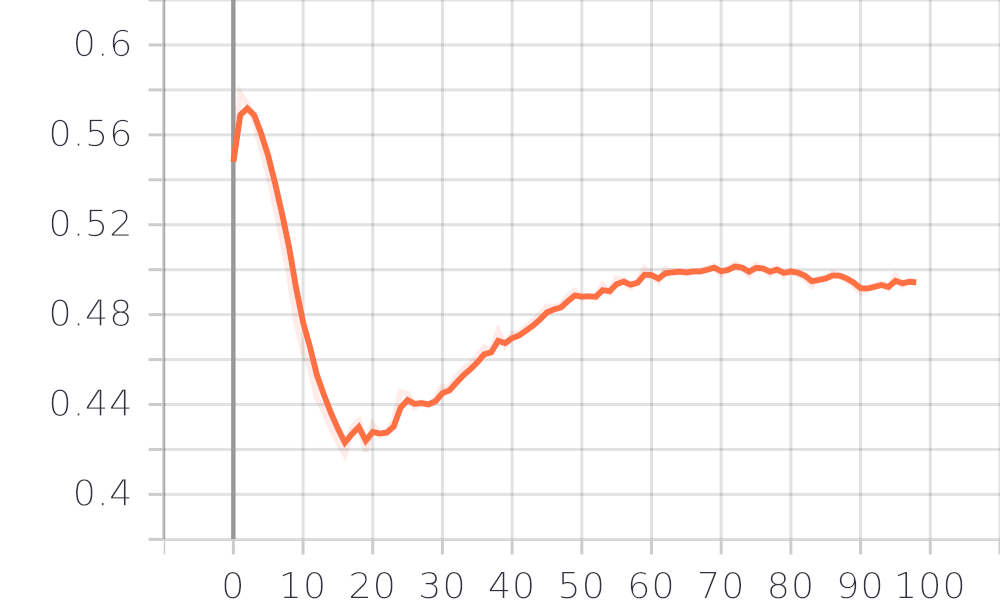
\includegraphics[width=\textwidth]{Discriminator_Loss_Real}
    \caption{Discriminator real loss over epochs}
  \end{minipage}
  \begin{minipage}[b]{0.4\textwidth}
    \centering
    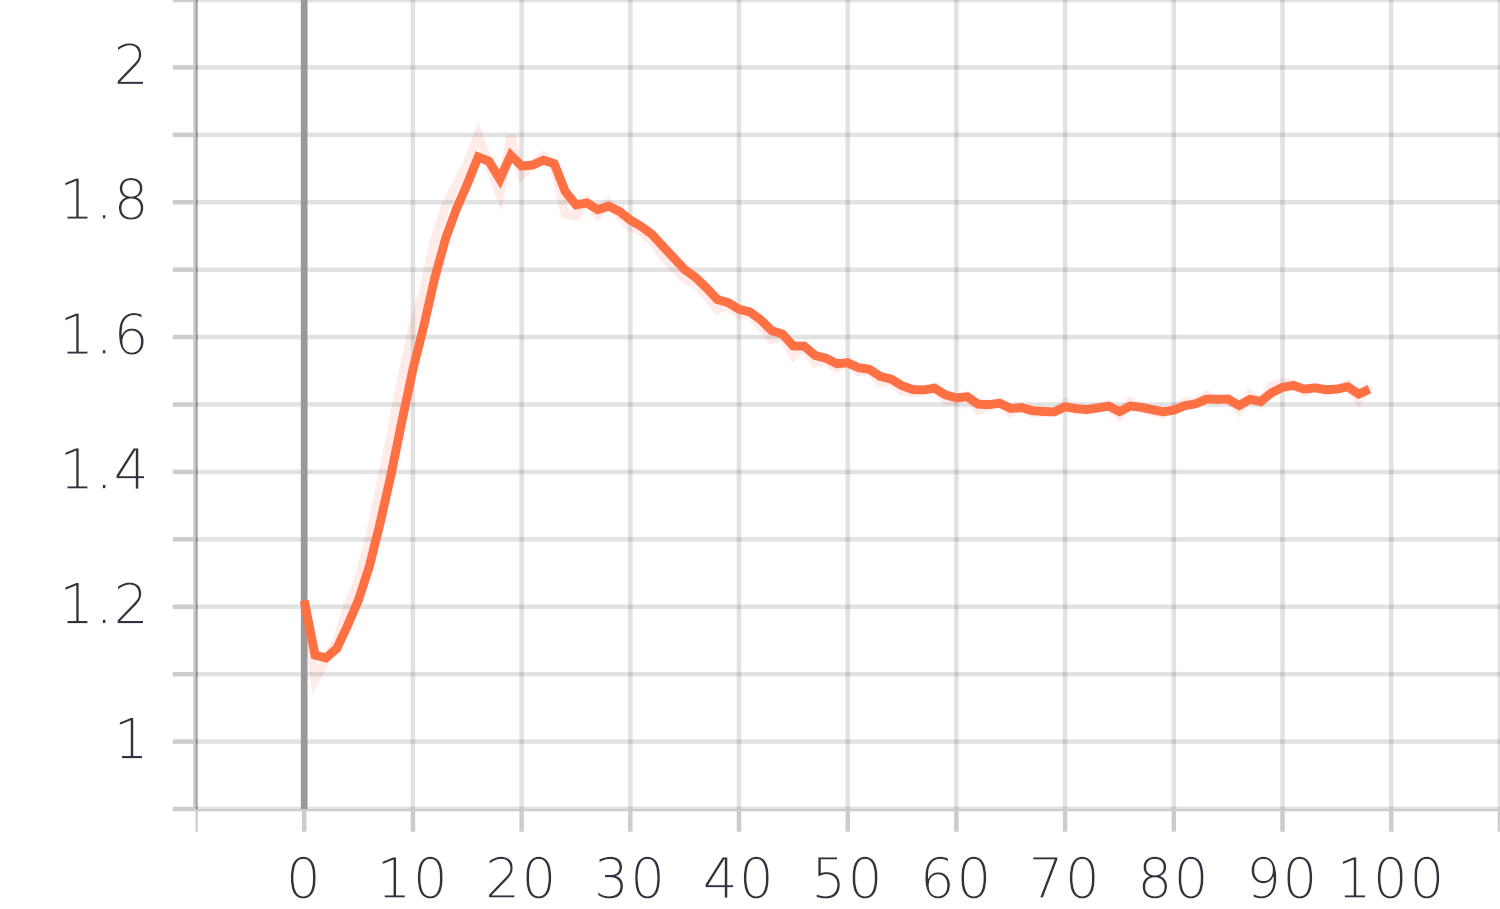
\includegraphics[width=\textwidth]{Generator_Loss}
    \caption{Generator loss over epochs}
  \end{minipage}
\end{figure}

After 100 epochs, the \ac{DCGAN} for MNIST number generation had an exceptionally good
performance when the generated images are displayed.
It is hard to tell if these are generated images or if they are part of the training set.
The generated images sometimes have a bit more of blur to them, but certainly with more epochs and more training samples this could be minimized.

\begin{figure}[H]
    \centering
    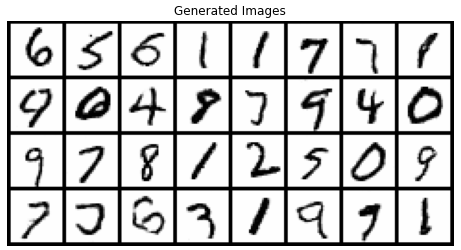
\includegraphics[width=0.6\textwidth]{gan_generated_images}
    \caption{GAN generated MNIST digits}
\end{figure}

%---}}}

% |--- Conclusion ---|----------------------{{{
\chapter{Conclusion}
%---}}}

% |--- References ---|----------------------{{{
\renewcommand\bibname{List of References}
\bibliography{references}
%---}}}

\end{document}
%===}}}
